% ****************************************************************************************
% ************************            PRACTICA 2              ****************************
% ****************************************************************************************


% =======================================================
% =======         HEADER FOR DOCUMENT        ============
% =======================================================
    
    % *********   HEADERS AND FOOTERS ********
    \def\ProjectAuthorLink{https://github.com/SoyOscarRH}           %Just to keep it in line
    \def\ProjectNameLink{\ProjectAuthorLink/Proyect}                %Link to Proyect

    % *********   DOCUMENT ITSELF   **************
    \documentclass[12pt, fleqn]{article}                             %Type of docuemtn and size of font and left eq
    \usepackage[spanish]{babel}                                     %Please use spanish
    \usepackage[utf8]{inputenc}                                     %Please use spanish - UFT
    \usepackage[margin = 0.9in]{geometry}                           %Margins and Geometry pacakge
    \usepackage{ifthen}                                             %Allow simple programming
    \usepackage{hyperref}                                           %Create MetaData for a PDF and LINKS!
    \usepackage{pdfpages}                                           %Create MetaData for a PDF and LINKS!
    \hypersetup{pageanchor = false}                                 %Solve 'double page 1' warnings in build
    \setlength{\parindent}{0pt}                                     %Eliminate ugly indentation
    \author{Oscar Andrés Rosas}                                     %Who I am

    % *********   LANGUAJE    *****************
    \usepackage[T1]{fontenc}                                        %Please use spanish
    \usepackage{textcmds}                                           %Allow us to use quoutes
    \usepackage{changepage}                                         %Allow us to use identate paragraphs
    \usepackage{anyfontsize}                                        %All the sizes

    % *********   MATH AND HIS STYLE  *********
    \usepackage{ntheorem, amsmath, amssymb, amsfonts}               %All fucking math, I want all!
    \usepackage{mathrsfs, mathtools, empheq}                        %All fucking math, I want all!
    \usepackage{cancel}                                             %Negate symbol
    \usepackage{centernot}                                          %Allow me to negate a symbol
    \decimalpoint                                                   %Use decimal point

    % *********   GRAPHICS AND IMAGES *********
    \usepackage{graphicx}                                           %Allow to create graphics
    \usepackage{float}                                              %For images
    \usepackage{wrapfig}                                            %Allow to create images
    \graphicspath{ {Graphics/} }                                    %Where are the images :D

    % *********   LISTS AND TABLES ***********
    \usepackage{listings, listingsutf8}                             %We will be using code here
    \usepackage[inline]{enumitem}                                   %We will need to enumarate
    \usepackage{tasks}                                              %Horizontal lists
    \usepackage{longtable}                                          %Lets make tables awesome
    \usepackage{booktabs}                                           %Lets make tables awesome
    \usepackage{tabularx}                                           %Lets make tables awesome
    \usepackage{multirow}                                           %Lets make tables awesome
    \usepackage{multicol}                                           %Create multicolumns

    % *********   HEADERS AND FOOTERS ********
    \usepackage{fancyhdr}                                           %Lets make awesome headers/footers
    \pagestyle{fancy}                                               %Lets make awesome headers/footers
    \setlength{\headheight}{16pt}                                   %Top line
    \setlength{\parskip}{0.5em}                                     %Top line
    \renewcommand{\footrulewidth}{0.5pt}                            %Bottom line

    \lhead{                                                         %Left Header
        \hyperlink{section.\arabic{section}}                        %Make a link to the current chapter
        {\normalsize{\textsc{\nouppercase{\leftmark}}}}             %And fot it put the name
    }

    \rhead{                                                         %Right Header
        \hyperlink{section.\arabic{section}.\arabic{subsection}}    %Make a link to the current chapter
            {\footnotesize{\textsc{\nouppercase{\rightmark}}}}      %And fot it put the name
    }

    \rfoot{\textsc{\small{\hyperref[sec:Index]{Ve al Índice}}}}     %This will always be a footer  

    \fancyfoot[L]{                                                  %Algoritm for a changing footer
        \ifthenelse{\isodd{\value{page}}}                           %IF ODD PAGE:
            {\footnotesize {\textsc{Practica 2}}}                   %Send the page
            {\footnotesize {\textsc{Algoritmos de Búsqueda}}}       %Send the page
    }
    
    
    
% =======================================================
% ===================   COMMANDS    =====================
% =======================================================

    % =========================================
    % =======   NEW ENVIRONMENTS   ============
    % =========================================
    \newenvironment{Indentation}[1][0.75em]                         %Use: \begin{Inde...}[Num]...\end{Inde...}
        {\begin{adjustwidth}{#1}{}}                                 %If you dont put nothing i will use 0.75 em
        {\end{adjustwidth}}                                         %This indentate a paragraph
    \newenvironment{SmallIndentation}[1][0.75em]                    %Use: The same that we upper one, just 
        {\begin{adjustwidth}{#1}{}\begin{footnotesize}}             %footnotesize size of letter by default
        {\end{footnotesize}\end{adjustwidth}}                       %that's it

    \newenvironment{MultiLineEquation}[1]                           %Use: To create MultiLine equations
        {\begin{equation}\begin{alignedat}{#1}}                     %Use: \begin{Multi..}{Num. de Columnas}
        {\end{alignedat}\end{equation}}                             %And.. that's it!
    \newenvironment{MultiLineEquation*}[1]                          %Use: To create MultiLine equations
        {\begin{equation*}\begin{alignedat}{#1}}                    %Use: \begin{Multi..}{Num. de Columnas}
        {\end{alignedat}\end{equation*}}                            %And.. that's it!
    

    % =========================================
    % == GENERAL TEXT & SYMBOLS ENVIRONMENTS ==
    % =========================================
    
    % =====  TEXT  ======================
    \newcommand \Quote {\qq}                                        %Use: \Quote to use quotes
    \newcommand \Over {\overline}                                   %Use: \Bar to use just for short
    \newcommand \ForceNewLine {$\Space$\\}                          %Use it in theorems for example

    % =====  SPACES  ====================
    \DeclareMathOperator \Space {\quad}                             %Use: \Space for a cool mega space
    \DeclareMathOperator \MegaSpace {\quad \quad}                   %Use: \MegaSpace for a cool mega mega space
    \DeclareMathOperator \MiniSpace {\;}                            %Use: \Space for a cool mini space
    
    % =====  MATH TEXT  =================
    \newcommand \Such {\MiniSpace | \MiniSpace}                     %Use: \Such like in sets
    \newcommand \Also {\MiniSpace \text{y} \MiniSpace}              %Use: \Also so it's look cool
    \newcommand \Remember[1]{\Space\text{\scriptsize{#1}}}          %Use: \Remember so it's look cool
    
    % =====  THEOREMS  ==================
    \newtheorem{Theorem}{Teorema}[section]                          %Use: \begin{Theorem}[Name]\label{Nombre}...
    \newtheorem{Corollary}{Colorario}[Theorem]                      %Use: \begin{Corollary}[Name]\label{Nombre}...
    \newtheorem{Lemma}[Theorem]{Lemma}                              %Use: \begin{Lemma}[Name]\label{Nombre}...
    \newtheorem{Definition}{Definición}[section]                    %Use: \begin{Definition}[Name]\label{Nombre}...
    \theoremstyle{break}                                            %THEOREMS START 1 SPACE AFTER

    % =====  LOGIC  =====================
    \newcommand \lIff    {\leftrightarrow}                          %Use: \lIff for logic iff
    \newcommand \lEqual  {\MiniSpace \Leftrightarrow \MiniSpace}    %Use: \lEqual for a logic double arrow
    \newcommand \lInfire {\MiniSpace \Rightarrow \MiniSpace}        %Use: \lInfire for a logic infire
    \newcommand \lLongTo {\longrightarrow}                          %Use: \lLongTo for a long arrow

    % =====  FAMOUS SETS  ===============
    \DeclareMathOperator \Naturals     {\mathbb{N}}                 %Use: \Naturals por Notation
    \DeclareMathOperator \Primes       {\mathbb{P}}                 %Use: \Primes por Notation
    \DeclareMathOperator \Integers     {\mathbb{Z}}                 %Use: \Integers por Notation
    \DeclareMathOperator \Racionals    {\mathbb{Q}}                 %Use: \Racionals por Notation
    \DeclareMathOperator \Reals        {\mathbb{R}}                 %Use: \Reals por Notation
    \DeclareMathOperator \Complexs     {\mathbb{C}}                 %Use: \Complex por Notation
    \DeclareMathOperator \GenericField {\mathbb{F}}                 %Use: \GenericField por Notation
    \DeclareMathOperator \VectorSet    {\mathbb{V}}                 %Use: \VectorSet por Notation
    \DeclareMathOperator \SubVectorSet {\mathbb{W}}                 %Use: \SubVectorSet por Notation
    \DeclareMathOperator \Polynomials  {\mathbb{P}}                 %Use: \Polynomials por Notation
    \DeclareMathOperator \VectorSpace  {\VectorSet_{\GenericField}} %Use: \VectorSpace por Notation
    \DeclareMathOperator \LinealTransformation {\mathcal{T}}        %Use: \LinealTransformation for a cool T
    \DeclareMathOperator \LinTrans {\mathcal{T}}                    %Use: \LinTrans for a cool T


    % =====  CONTAINERS   ===============
    \newcommand{\Set}[1]    {\left\{ \; #1 \; \right\}}             %Use: \Set {Info} for INTELLIGENT space 
    \newcommand{\bigSet}[1] {\big\{  \; #1 \; \big\}}               %Use: \bigSet  {Info} for space 
    \newcommand{\BigSet}[1] {\Big\{  \; #1 \; \Big\}}               %Use: \BigSet  {Info} for space 
    \newcommand{\biggSet}[1]{\bigg\{ \; #1 \; \bigg\}}              %Use: \biggSet {Info} for space 
    \newcommand{\BiggSet}[1]{\Bigg\{ \; #1 \; \Bigg\}}              %Use: \BiggSet {Info} for space 
    
    \newcommand{\Brackets}[1]    {\left[ #1 \right]}                %Use: \Brackets {Info} for INTELLIGENT space
    \newcommand{\bigBrackets}[1] {\big[ \; #1 \; \big]}             %Use: \bigBrackets  {Info} for space 
    \newcommand{\BigBrackets}[1] {\Big[ \; #1 \; \Big]}             %Use: \BigBrackets  {Info} for space 
    \newcommand{\biggBrackets}[1]{\bigg[ \; #1 \; \bigg]}           %Use: \biggBrackets {Info} for space 
    \newcommand{\BiggBrackets}[1]{\Bigg[ \; #1 \; \Bigg]}           %Use: \BiggBrackets {Info} for space 
    
    \newcommand{\Wrap}[1]    {\left( #1 \right)}                    %Use: \Wrap {Info} for INTELLIGENT space
    \newcommand{\bigWrap}[1] {\big( \; #1 \; \big)}                 %Use: \bigBrackets  {Info} for space 
    \newcommand{\BigWrap}[1] {\Big( \; #1 \; \Big)}                 %Use: \BigBrackets  {Info} for space 
    \newcommand{\biggWrap}[1]{\bigg( \; #1 \; \bigg)}               %Use: \biggBrackets {Info} for space 
    \newcommand{\BiggWrap}[1]{\Bigg( \; #1 \; \Bigg)}               %Use: \BiggBrackets {Info} for space 
    
    \newcommand{\Generate}[1]{\left\langle #1 \right\rangle}        %Use: \Generate {Info} <>
    \newcommand{\Floor}[1]{\left \lfloor #1 \right \rfloor}         %Use: \Floor {Info} for floor 
    \newcommand{\Ceil}[1]{\left \lceil #1 \right \rceil }           %Use: \Ceil {Info} for ceil
    
    % =====  BETTERS MATH COMMANDS   =====
    \newcommand{\pfrac}[2]{\Wrap{\dfrac{#1}{#2}}}                   %Use: Put fractions in parentesis

    % =========================================
    % ====   LINEAL ALGEBRA & VECTORS    ======
    % =========================================

    % ===== UNIT VECTORS  ================
    \newcommand{\hati} {\hat{\imath}}                               %Use: \hati for unit vector    
    \newcommand{\hatj} {\hat{\jmath}}                               %Use: \hatj for unit vector    
    \newcommand{\hatk} {\hat{k}}                                    %Use: \hatk for unit vector

    % ===== FN LINEAL TRANSFORMATION  ====
    \newcommand{\FnLinTrans}[1]{\mathcal{T}\Wrap{#1}}               %Use: \FnLinTrans for a cool T
    \newcommand{\VecLinTrans}[1]{\mathcal{T}\pVector{#1}}           %Use: \LinTrans for a cool T
    \newcommand{\FnLinealTransformation}[1]{\mathcal{T}\Wrap{#1}}   %Use: \FnLinealTransformation

    % ===== MAGNITUDE  ===================
    \newcommand{\abs}[1]{\left\lvert #1 \right\lvert}               %Use: \abs{expression} for |x|
    \newcommand{\Abs}[1]{\left\lVert #1 \right\lVert}               %Use: \Abs{expression} for ||x||
    \newcommand{\Mag}[1]{\left| #1 \right|}                         %Use: \Mag {Info} 
    
    \newcommand{\bVec}[1]{\mathbf{#1}}                              %Use for bold type of vector
    \newcommand{\lVec}[1]{\overrightarrow{#1}}                      %Use for a long arrow over a vector
    \newcommand{\uVec}[1]{\mathbf{\hat{#1}}}                        %Use: Unitary Vector Example: $\uVec{i}

    % ===== ALL FOR DOT PRODUCT  =========
    \makeatletter                                                   %WTF! IS THIS
    \newcommand*\dotP{\mathpalette\dotP@{.5}}                       %Use: \dotP for dot product
    \newcommand*\dotP@[2] {\mathbin {                               %WTF! IS THIS            
        \vcenter{\hbox{\scalebox{#2}{$\m@th#1\bullet$}}}}           %WTF! IS THIS
    }                                                               %WTF! IS THIS
    \makeatother                                                    %WTF! IS THIS

    % === WRAPPERS FOR COLUMN VECTOR ===
    \newcommand{\pVector}[1]                                        %Use: \pVector {Matrix Notation} use parentesis
        { \ensuremath{\begin{pmatrix}#1\end{pmatrix}} }             %Example: \pVector{a\\b\\c} or \pVector{a&b&c} 
    \newcommand{\lVector}[1]                                        %Use: \lVector {Matrix Notation} use a abs 
        { \ensuremath{\begin{vmatrix}#1\end{vmatrix}} }             %Example: \lVector{a\\b\\c} or \lVector{a&b&c} 
    \newcommand{\bVector}[1]                                        %Use: \bVector {Matrix Notation} use a brackets 
        { \ensuremath{\begin{bmatrix}#1\end{bmatrix}} }             %Example: \bVector{a\\b\\c} or \bVector{a&b&c} 
    \newcommand{\Vector}[1]                                         %Use: \Vector {Matrix Notation} no parentesis
        { \ensuremath{\begin{matrix}#1\end{matrix}} }               %Example: \Vector{a\\b\\c} or \Vector{a&b&c}

    % === MAKE MATRIX BETTER  =========
    \makeatletter                                                   %Example: \begin{matrix}[cc|c]
    \renewcommand*\env@matrix[1][*\c@MaxMatrixCols c] {             %WTF! IS THIS
        \hskip -\arraycolsep                                        %WTF! IS THIS
        \let\@ifnextchar\new@ifnextchar                             %WTF! IS THIS
        \array{#1}                                                  %WTF! IS THIS
    }                                                               %WTF! IS THIS
    \makeatother                                                    %WTF! IS THIS

    % =========================================
    % =======   FAMOUS FUNCTIONS   ============
    % =========================================

    % == TRIGONOMETRIC FUNCTIONS  ====
    \newcommand{\Cos}[1] {\cos\Wrap{#1}}                            %Simple wrappers
    \newcommand{\Sin}[1] {\sin\Wrap{#1}}                            %Simple wrappers
    \newcommand{\Tan}[1] {tan\Wrap{#1}}                             %Simple wrappers
    
    \newcommand{\Sec}[1] {sec\Wrap{#1}}                             %Simple wrappers
    \newcommand{\Csc}[1] {csc\Wrap{#1}}                             %Simple wrappers
    \newcommand{\Cot}[1] {cot\Wrap{#1}}                             %Simple wrappers

    % === COMPLEX ANALYSIS TRIG ======
    \newcommand \Cis[1]  {\Cos{#1} + i \Sin{#1}}                    %Use: \Cis for cos(x) + i sin(x)
    \newcommand \pCis[1] {\Wrap{\Cis{#1}}}                          %Use: \pCis for the same with parantesis
    \newcommand \bCis[1] {\Brackets{\Cis{#1}}}                      %Use: \bCis for the same with Brackets


    % =========================================
    % ===========     CALCULUS     ============
    % =========================================

    % ====== TRANSFORMS =============
    \newcommand{\FourierT}[1]{\mathscr{F} \left\{ #1 \right\} }     %Use: \FourierT {Funtion}
    \newcommand{\InvFourierT}[1]{\mathscr{F}^{-1}\left\{#1\right\}} %Use: \InvFourierT {Funtion}

    % ====== DERIVATIVES ============
    \newcommand \MiniDerivate[1][x] {\dfrac{d}{d #1}}               %Use: \MiniDerivate[var] for simple use [var]
    \newcommand \Derivate[2] {\dfrac{d \; #1}{d #2}}                %Use: \Derivate [f(x)][x]
    \newcommand \MiniUpperDerivate[2] {\dfrac{d^{#2}}{d#1^{#2}}}    %Mini Derivate High Orden Derivate -- [x][pow]
    \newcommand \UpperDerivate[3] {\dfrac{d^{#3} \; #1}{d#2^{#3}}}  %Complete High Orden Derivate -- [f(x)][x][pow]
    
    \newcommand \MiniPartial[1][x] {\dfrac{\partial}{\partial #1}}  %Use: \MiniDerivate for simple use [var]
    \newcommand \Partial[2] {\dfrac{\partial \; #1}{\partial #2}}   %Complete Partial Derivate -- [f(x)][x]
    \newcommand \MiniUpperPartial[2]                                %Mini Derivate High Orden Derivate -- [x][pow] 
        {\dfrac{\partial^{#2}}{\partial #1^{#2}}}                   %Mini Derivate High Orden Derivate
    \newcommand \UpperPartial[3]                                    %Complete High Orden Derivate -- [f(x)][x][pow]
        {\dfrac{\partial^{#3} \; #1}{\partial#2^{#3}}}              %Use: \UpperDerivate for simple use

    \DeclareMathOperator \Evaluate  {\Big|}                         %Use: \Evaluate por Notation

    % =========================================
    % ========    GENERAL STYLE     ===========
    % =========================================
    
    % =====  COLORS ==================
    \definecolor{RedMD}{HTML}{F44336}                               %Use: Color :D        
    \definecolor{Red100MD}{HTML}{FFCDD2}                            %Use: Color :D        
    \definecolor{Red200MD}{HTML}{EF9A9A}                            %Use: Color :D        
    \definecolor{Red300MD}{HTML}{E57373}                            %Use: Color :D        
    \definecolor{Red700MD}{HTML}{D32F2F}                            %Use: Color :D 

    \definecolor{PurpleMD}{HTML}{9C27B0}                            %Use: Color :D        
    \definecolor{Purple100MD}{HTML}{E1BEE7}                         %Use: Color :D        
    \definecolor{Purple200MD}{HTML}{EF9A9A}                         %Use: Color :D        
    \definecolor{Purple300MD}{HTML}{BA68C8}                         %Use: Color :D        
    \definecolor{Purple700MD}{HTML}{7B1FA2}                         %Use: Color :D 

    \definecolor{IndigoMD}{HTML}{3F51B5}                            %Use: Color :D        
    \definecolor{Indigo100MD}{HTML}{C5CAE9}                         %Use: Color :D        
    \definecolor{Indigo200MD}{HTML}{9FA8DA}                         %Use: Color :D        
    \definecolor{Indigo300MD}{HTML}{7986CB}                         %Use: Color :D        
    \definecolor{Indigo700MD}{HTML}{303F9F}                         %Use: Color :D 

    \definecolor{BlueMD}{HTML}{2196F3}                              %Use: Color :D        
    \definecolor{Blue100MD}{HTML}{BBDEFB}                           %Use: Color :D        
    \definecolor{Blue200MD}{HTML}{90CAF9}                           %Use: Color :D        
    \definecolor{Blue300MD}{HTML}{64B5F6}                           %Use: Color :D        
    \definecolor{Blue700MD}{HTML}{1976D2}                           %Use: Color :D        
    \definecolor{Blue900MD}{HTML}{0D47A1}                           %Use: Color :D  

    \definecolor{CyanMD}{HTML}{00BCD4}                              %Use: Color :D        
    \definecolor{Cyan100MD}{HTML}{B2EBF2}                           %Use: Color :D        
    \definecolor{Cyan200MD}{HTML}{80DEEA}                           %Use: Color :D        
    \definecolor{Cyan300MD}{HTML}{4DD0E1}                           %Use: Color :D        
    \definecolor{Cyan700MD}{HTML}{0097A7}                           %Use: Color :D        
    \definecolor{Cyan900MD}{HTML}{006064}                           %Use: Color :D 

    \definecolor{TealMD}{HTML}{009688}                              %Use: Color :D        
    \definecolor{Teal100MD}{HTML}{B2DFDB}                           %Use: Color :D        
    \definecolor{Teal200MD}{HTML}{80CBC4}                           %Use: Color :D        
    \definecolor{Teal300MD}{HTML}{4DB6AC}                           %Use: Color :D        
    \definecolor{Teal700MD}{HTML}{00796B}                           %Use: Color :D        
    \definecolor{Teal900MD}{HTML}{004D40}                           %Use: Color :D 

    \definecolor{GreenMD}{HTML}{4CAF50}                             %Use: Color :D        
    \definecolor{Green100MD}{HTML}{C8E6C9}                          %Use: Color :D        
    \definecolor{Green200MD}{HTML}{A5D6A7}                          %Use: Color :D        
    \definecolor{Green300MD}{HTML}{81C784}                          %Use: Color :D        
    \definecolor{Green700MD}{HTML}{388E3C}                          %Use: Color :D        
    \definecolor{Green900MD}{HTML}{1B5E20}                          %Use: Color :D

    \definecolor{AmberMD}{HTML}{FFC107}                             %Use: Color :D        
    \definecolor{Amber100MD}{HTML}{FFECB3}                          %Use: Color :D        
    \definecolor{Amber200MD}{HTML}{FFE082}                          %Use: Color :D        
    \definecolor{Amber300MD}{HTML}{FFD54F}                          %Use: Color :D        
    \definecolor{Amber700MD}{HTML}{FFA000}                          %Use: Color :D        
    \definecolor{Amber900MD}{HTML}{FF6F00}                          %Use: Color :D

    \definecolor{BlueGreyMD}{HTML}{607D8B}                          %Use: Color :D        
    \definecolor{BlueGrey100MD}{HTML}{CFD8DC}                       %Use: Color :D        
    \definecolor{BlueGrey200MD}{HTML}{B0BEC5}                       %Use: Color :D        
    \definecolor{BlueGrey300MD}{HTML}{90A4AE}                       %Use: Color :D        
    \definecolor{BlueGrey700MD}{HTML}{455A64}                       %Use: Color :D        
    \definecolor{BlueGrey900MD}{HTML}{263238}                       %Use: Color :D        

    \definecolor{DeepPurpleMD}{HTML}{673AB7}                        %Use: Color :D

    \newcommand{\Color}[2]{\textcolor{#1}{#2}}                     %Simple color environment
    \newenvironment{ColorText}[1]                                   %Use: \begin{ColorText}
        { \leavevmode\color{#1}\ignorespaces }                      %That's is!

    % =====  CODE EDITOR =============
    \lstdefinestyle{CompilandoStyle} {                              %This is Code Style
        backgroundcolor     = \color{BlueGrey900MD},                %Background Color  
        basicstyle          = \tiny\color{BlueGrey900MD},           %Style of text
        commentstyle        = \color{BlueGrey300MD},                %Comment style
        stringstyle         = \color{Green300MD},                   %String style
        keywordstyle        = \color{Blue300MD},                    %keywords style
        numberstyle         = \tiny\color{TealMD},                  %Size of a number
        frame               = shadowbox,                            %Adds a frame around the code
        breakatwhitespace   = true,                                 %Style   
        breaklines          = true,                                 %Style   
        showstringspaces    = false,                                %Hate those spaces                  
        breaklines          = true,                                 %Style                   
        keepspaces          = true,                                 %Style                   
        numbers             = left,                                 %Style                   
        numbersep           = 10pt,                                 %Style 
        xleftmargin         = \parindent,                           %Style 
        tabsize             = 4,                                    %Style
        inputencoding       = utf8/latin1                           %Allow me to use special chars
    }

    % =====  CODE EDITOR =============
    \lstdefinestyle{CompilandoStylePurity} {                        %This is Code Style
        backgroundcolor     = \color{white},                        %Background Color  
        basicstyle          = \tiny\color{BlueGrey900MD},           %Style of text
        commentstyle        = \color{Green300MD},                   %Comment style
        stringstyle         = \color{Teal700MD},                    %String style
        keywordstyle        = \color{Blue700MD},                    %keywords style
        numberstyle         = \tiny\color{TealMD},                  %Size of a number
        frame               = none,                                 %Adds a frame around the code
        breakatwhitespace   = true,                                 %Style   
        breaklines          = true,                                 %Style   
        showstringspaces    = false,                                %Hate those spaces                  
        breaklines          = true,                                 %Style                   
        keepspaces          = true,                                 %Style                   
        numbers             = left,                                 %Style                   
        numbersep           = 11pt,                                 %Style 
        xleftmargin         = \parindent,                           %Style 
        tabsize             = 4,                                    %Style
        inputencoding       = utf8/latin1                           %Allow me to use special chars
    }
 
    \lstset{style = CompilandoStylePurity}                          %Use this style











\usepackage{algpseudocode}  %Los 2 paquetes son para poner pseudocodigo 
\usepackage{algorithm}
\usepackage{dirtree}
\algdef{SE}[DOWHILE]{Do}{doWhile}{\algorithmicdo}[1]{\algorithmicwhile\ #1}






% =====================================================
% ============        COVER PAGE       ================
% =====================================================
\begin{document}
\begin{titlepage}

    \center
    % ============ UNIVERSITY NAME AND DATA =========
    \textsc{\Large Instituto Politécnico Nacional \\ Escuela Superior de Cómputo}\\[0.5cm] 
    \textsc{\large Análisis de Algoritmos}\\[1.5cm]

    % ============ NAME OF THE DOCUMENT  ============
    \rule{\linewidth}{0.5mm} \\[1.0cm]
        { \huge \bfseries Práctica 2: Pruebas a Posteriori (Algoritmos de Búsqueda)}\\[1.0cm] 
    \rule{\linewidth}{0.5mm} \\[1.5cm]
     
    % ============  MY INFORMATION  =================
    \textbf{\textsc{Equipo:}}       \\
    CompilandoConocimiento          \\[1cm]

    \begin{minipage}{0.4\textwidth}
        \begin{flushleft} \large

            \textbf{\textsc{Integrantes:}}      \\
            \small{
                Morales López Laura Andrea      \\
                Ontiveros Salazar Alan Enrique  \\
                Rosas Hernández Óscar Andrés
            }
        \end{flushleft}
    \end{minipage}
    ~
    \begin{minipage}{0.4\textwidth}
        \begin{flushright} \large
            \textbf{\textsc{Profesor: }}\\
            Franco Martínez Edgardo Adrián
        \end{flushright}
    \end{minipage}\\[1.5cm]

    \begin{figure}[h]
        \centering
        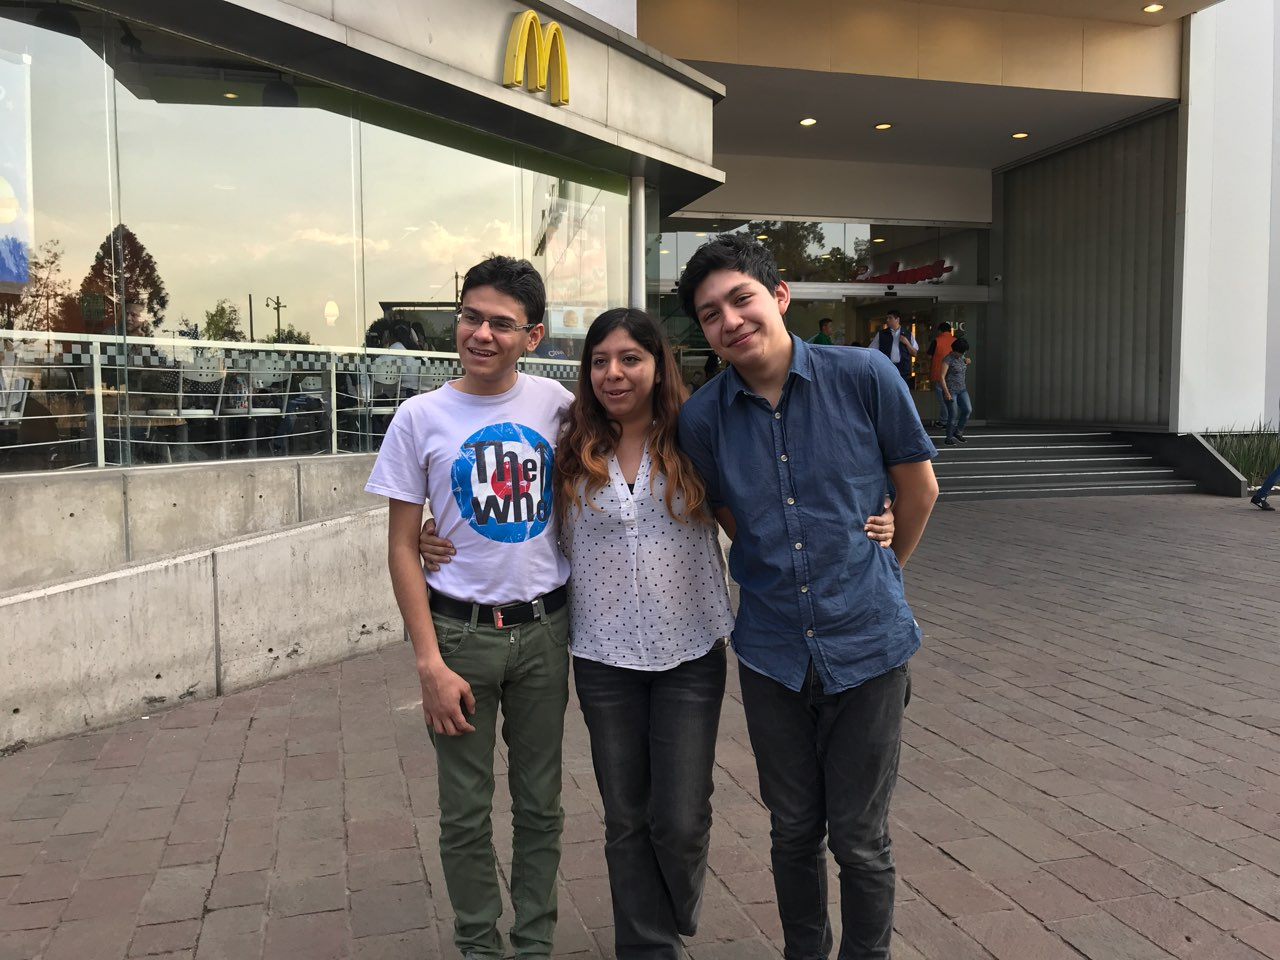
\includegraphics[width=0.55\textwidth]{Foto}
    \end{figure}

    \vfill

\end{titlepage}

% =====================================================
% ==========      RESTORE TO DOCUMENT      ============
% =====================================================
\restoregeometry                                                    %Restores the geometry
\nopagecolor                                                        %Use to restore the color to white




% =====================================================
% ========                INDICE              =========
% =====================================================
\tableofcontents{}
\label{sec:Index}




% ===============================================================================
% ===================          INTRODUCCIÓN                ======================
% ===============================================================================
\clearpage
\section{Introducción}


    Uno de los típicos problemas dentro de un curso de programación es la búsqueda.
    Estos algoritmos son la base de muchos otros, además de que tenemos con ellos unas ideas
    interesantes a usar en otro tipo de algoritmos, como búsqueda binarai y derivados, las
    estructuras de datos y los algoritmos concurrentes.

    % ===============================================================
    % ==================       METODOS         ======================
    % ===============================================================
    \subsection{Métodos}

    % ===============================================================
    % ==================       DEFINICION      ======================
    % ===============================================================
    \subsection{Definición}


    % ===============================================================
    % ===========      ALGORITMOS DE BUSQUEDA      ==================
    % ===============================================================
    \subsection{Algoritmos de Búsqueda}




% ===============================================================================
% ===========          PLANTEAMIENTO DEL PROBLEMA          ======================
% ===============================================================================
\clearpage
\section{Planteamiento del Problema}


    Con base en el ordenamiento obtenido a partir del archivo de entrada de la práctica
    1 que tiene 10 millones de números diferentes; realizar la búsqueda de elementos
    bajo tres métodos de búsqueda, realizar el análisis teórico y experimental
    de las complejidades, así como encontrar las cotas de los algoritmos.
    
    \begin{enumerate}\setlength\itemsep{0em}
        \item Búsqueda lineal o secuencial
        \item Búsqueda binaria o dicotómica
        \item Búsqueda en un árbol binario de búsqueda
        \item Implementación de las tres búsquedas con Threads
    \end{enumerate}


% ===============================================================================
% =================         DISEÑO DE LA SOLUCION          ======================
% ===============================================================================
\clearpage
\section{Diseño de la Solución}

    \subsection{Búsqueda Lineal}
        \begin{algorithm}[H]
        \caption{LinealSearch}
        \begin{algorithmic}[1]
            \Procedure{LinealSearch}{$A, n, NumberToSearch$}
            \For{$i \gets 0$ hasta $n$}
                \If{$A[i] = NumberToSearch$}
                    \State regresa i
                \EndIf
            \EndFor

            regresa -1
            \EndProcedure
            \end{algorithmic}
        \end{algorithm}
        
    \subsection{Búsqueda Binaria}
        \begin{algorithm}[H]
        \caption{BinarySearch}
        \begin{algorithmic}[1]
            \Procedure{BinarySearch}{$A, n, NumberToSearch$}
            \State $inicio \gets 0$
            \State $final \gets n$
            \While{inicio $\leq$ final}
               \State medio $\gets$ inicio + ((final - inicio) / 2)
                \If{$A[medio] = NumberToSearch$}
                    \State regresa medio
                \EndIf
                \If{$A[medio] > NumberToSearch$}
                    \State final $\gets$ medio -1
                \EndIf
                \If{$A[medio] > NumberToSearch$}
                    \State inicio $\gets$ medio + 1
                \EndIf
            \EndWhile
            regresa -1
            \EndProcedure
            \end{algorithmic}
        \end{algorithm}
        
    \subsection{Búsqueda con BTS}
        \begin{algorithm}[H]
        \caption{SearchBTS}
        \begin{algorithmic}[1]
            \Procedure{SearchBTS}{$A, n, NumberToSearch$}
            \State arbol $\gets$ CreaArbol(A, n)
            \State nodo $\gets$ Raiz del árbol
            \While{nodo no sea nulo}
                \If{nodo.informacion = NumberToSearch}
                    \State nodo.indice
                \EndIf
                \If{NumberToSearch < nodo.informacion}
                    \State nodo $\gets$ nodo.derecha
                \EndIf
                \If{NumberToSearch > nodo.informacion}
                    \State nodo $\gets$ nodo.izquierda
                \EndIf
            \EndWhile
            regresa -1
            \EndProcedure
            \end{algorithmic}
        \end{algorithm}




% ===============================================================================
% ============          IMPLEMENTEACION DE LA SOLUCION           ================
% ===============================================================================
\clearpage
\section{Implementación de la Solución}

    % ===============================================================
    % ============          BUSQUEDA LINEAL           ===============
    % ===============================================================
    \clearpage
    \subsection{Búsqueda Lineal}

        \lstinputlisting[language=C, linerange={14-34}, gobble=8]{Code/LinealSearch.c}

    % ===============================================================
    % =========     BUSQUEDA LINEAL PARALELA          ===============
    % ===============================================================
    \clearpage
    \subsection{Búsqueda Lineal Paralela}
        \lstinputlisting[language=C, linerange={37-114}, gobble=8]{Code/LinealSearch.c}

    % ===============================================================
    % ============          BUSQUEDA BINARIA          ===============
    % ===============================================================
    \clearpage
    \subsection{Búsqueda Binaria}

        \lstinputlisting[language=C, linerange={1-29}, gobble=8]{Code/BinarySearch.c}

    % ===============================================================
    % =========     BUSQUEDA BINARIA PARALELA          ===============
    % ===============================================================
    \clearpage
    \subsection{Búsqueda Binaria Paralela}
        \lstinputlisting[language=C, linerange={44-115}, gobble=8]{Code/BinarySearch.c}

    % ===============================================================
    % =========     BUSQUEDA CON BTS                  ===============
    % ===============================================================
    \clearpage
    \subsection{Búsqueda con BTS}
        \lstinputlisting[language=C, linerange={16-40}, gobble=8]{Code/SearchInBST.c}





% ===============================================================================
% ===================         ACTIVIDADES Y PRUEBA         ======================
% ===============================================================================
\clearpage
\section{Actividades y Pruebas}


    % ===============================================================
    % ===========      COMPARATIVAS INDIVIDUALES      ===============
    % ===============================================================
    \subsection{Comparativas Individuales}


    % ===============================================================
    % ===========      COMPARATIVAS GLOBALES          ===============
    % ===============================================================
    \subsection{Comparativas Globales}


    % ===============================================================
    % ===========               PREGUNTAS             ===============
    % ===============================================================
    \subsection{Preguntas}


        \begin{itemize}
            \item 
                \textbf{¿Cuál de los 3 algoritmos es más fácil de implementar?}

                El más sencillo (o en algoritmia conocido coloquialmente como la bruta)
                es la búsqueda lineal. Es la solución más sencilla con apenas 3 o 4 líneas de código.

                Además de ser sencilla de implementar es en la que puedes cometer un error con menor
                probabilidad a la hora de definir los índices o variables de apoyo.

            \item 
                \textbf{¿Cuál de los 3 algoritmos es el más difícil de implementar?}

                El más difícil de implementar en la búsqueda usando un Binary Search Tree, porque
                nos obliga a diseñar algoritmos que son comúnmente recursivos en algo
                iterativo.

            \item
                \textbf{¿Cuál de los 3 algoritmos es el más difícil de implementar en su variante
                con hilos?}

                Curiosamente la respuesta creo que tiene que ir para la versión con hilos de la búsqueda
                lineal.

                Por un lado el trabajar con hilos siempre complica las cosas, sobretodo porque involucra
                problemas de sincronicidad y el manejo de variables que pueden ser posiblemente accedidas
                por varios hilos. Aquí hay una consideración importante que hay que hacer:
                Solo estamos buscando una variable, por lo que no me tengo que preocupar con la memoria: 
                el primer hilo que me mande una respuesta, esa la tomaré y todos los demás hilos al notar
                el cambio en la variable se matan.

            \item
                \textbf{¿Cuál de los 3 algoritmos en su variante con hilos resulto ser mas rápido?}

                La búsqueda binaria, es cierto, que fue más rápida la versión lineal, pero aún así
                la versión con hilos es endemoniadamente rápida.

            \item
                \textbf{¿Cuál algoritmo tiene menor complejidad temporal?}

                La búsqueda binaria. Es uno de los algoritmos más famosos por tener un $O(\log_2(n))$
                aunque en ciertos casos, CON UN ÁRBOL BALANCEADO la búsqueda con árbol puede tener esa
                complejidad.

            \clearpage

            \item
                \textbf{¿Cuál algoritmo tiene mayor complejidad temporal?}

                Sin duda alguna ese premio tiene que ir para la búsqueda lineal, en el peor de los casos
                tenemos un búsqueda de $O(n)$.
            \item
                \textbf{¿El comportamiento experimental de los algoritmos era el esperado? ¿Por qué?}

                Sí, al menos en rangos generales de los algoritmos se esperaba y se ve la gran diferencia entre
                los algoritmos de búsqueda rápidos y la búsqueda lineal.

                Por otro lado a simple vista uno puede pensar que una variante con hilos siempre será más rápida
                que una versión que no es concurrente, pero esto no tiene porque ser así, por ejemplo
                en la búsqueda binaria es más que obvio que como solo estamos haciendo serie de comparaciones
                entonces el añadir hilos no mejora nada y solo sobrecarga al sistema operativo con su creación.

            \item
                \textbf{¿Sus resultados experimentales difieren mucho de los análisis teóricos
                    que realizó? ¿A que se debe?}

                No, como continuación de la respuesta anterior, si se analizaban con algo de tranquilidad
                los algoritmos se podía llegar a unas muy buenas estimaciones.

            \item
                \textbf{¿Los resultados experimentales de las implementación con hilos de los
                algoritmos realmente tardaron $\dfrac{F(t)}{\#hilos}$ de su implementación sin hilos?}

                Jajaja, si hablamos de la búsqueda lineal, claro, es decir, no fue exactamente esa cantidad
                sobretodo por los grandes márgenes de error que tenemos a la hora de medir tiempos
                tan pequeños pero el punto es que sí, casi casi tenemos una mejora linealmente correspondiente
                con la cantidad de hilos, después de todo dividimos el trabajo entre la cantidad de hilos.

                Pero en los otros dos al ser escencialemente una gran cantidad de comparaciones en lineal
                entonces no podemos llegar a prácticamente ninguna mejora, incluso un desempeño un poco peor.

                En general, para $n$ hilos tenemos una nueva función complejidad:
                \begin{itemize}
                    \item Búsqueda Lineal: $f_h(t) = \frac{f(t)}{\text{Número de hilos}}$
                    \item Búsqueda Binaria: $f_h(t) = 1 f(t)$
                    \item Búsqueda BST: $f_h(t) = 1 f(t)$
                \end{itemize}
                
            \item
                \textbf{¿Cuál es el \% de mejora que tiene cada uno de los algoritmos en su
                variante con hilos? ¿Es lo que esperabas? ¿Por qué?}

            \clearpage

            \item
                \textbf{¿Existió un entorno controlado para realizar las pruebas experimentales?
                ¿Cuál fue?}

                Sí, usamos una PC con las siguientes características:
                \begin{itemize}\setlength\itemsep{0em}
                    \item HP EliteDesk 700 G1 SFF
                    \item 8GB de memoria RAM, DDR3 SDRAM non-ECC, 1600MHz
                    \item Procesador Intel(R) Core(TM) i5-4590 (4$^\circ$ generación), CPU @ 3.30GHz 
                        (4 CPUs), $\sim$3.3GHz. Intel vPro Technology
                    \item 1TB de disco duro HDD, Serial ATA-600 6Gb/s, 7200 rpm
                \end{itemize}
                
                Y el software fue el siguiente:
                \begin{itemize}\setlength\itemsep{0em}
                    \item Sistema operativo Linux
                    \item Distribución Elementary OS 0.4
                    \item Compliador GCC con soporte para C11
                    \item Python 3.6 con las bibliotecas \texttt{matplotlib} y \texttt{numpy}
                    \item No había ninguna aplicación abierta al momento de ejecutar los algoritmos
                \end{itemize}

            \item
                \textbf{Si solo se realizara el análisis teórico de un algoritmo antes de
                implementarlo, ¿podrías asegurar cual es el mejor?}

                Con un análisis básico, es decir, con el uso de cotas, rápidamente podríamos descartar a
                la búsqueda lineal SI ES QUE NUESTRO ARREGLO ESTUVIERA ORDENADO; y ya que el BST
                requiere otro tiempo inicial para la creación del árbol, sería fácil decantarse por
                la sencilla búsqueda binaria.

                Pero si tenemos un arreglo que no está ordenado las cosas cambian, ahí depende mucho
                del tamaño del problema y de la cantidad de hilos que podemos correr eficientemente
                lo que decanta la balanza por BST o un búsqueda lineal.

            \item
                \textbf{¿Qué tan difícil fue realizar el análisis teórico de cada algoritmo?}

                \begin{itemize}
                    \item Búsqueda Lineal: Sencillo, de esos que son ejemplos básicos en clase.
                    \item Búsqueda Binaria: Algo más compleja, sobretodo por el cálculo de los
                    valores límites, pero la verdad es que no hay mucho más allá.
                    \item Búsqueda BST: Igualmente, el peor caso en un árbol BALANCEADO es bastante sencillo
                    de obtener.

                \end{itemize}

            \clearpage

            \item 
                \textbf{¿Qué recomendaciones darían a nuevos equipos para realizar esta práctica?}
                
                \begin{itemize}\setlength\itemsep{0em}
                    \item Hagan sus scripts jóvenes, pues aunque parezca más tedioso y crean que es más rápido
                        anotar toda la información solicitada (que es mucha) a mano, es más eficiente por si se
                        requiere cambiar algún algoritmo o los valores de entrada. Al menos que el script guarde
                        los tiempos en algún archivo de texto con un formato que quieran.
                    \item Prueben sus algoritmos con arreglos pequeños antes de buscar en los 10 millones para ver
                        si realmente los programaron bien.
                    \item Hagan sus programas generales, es decir, que reciban cualquier tamaño de subarreglo y
                        el algoritmo a usar.
                    \item Usen Linux, pues en Windows no están las bibliotecas para medir los tres tiempos.
                    \item Cuando corran sus algoritmos, procuren cerrar todas las tareas en segundo plano para
                        que los tiempos obtenidos sean lo más apegados a la realidad posible.
                \end{itemize}

        \end{itemize}




% ===============================================================================
% ===================         ERRORES DETECTADOS           ======================
% ===============================================================================
\clearpage
\section{Errores Detectados}

    Por un lado, no hemos detectado errores al momento de correr los algoritmos
    que no hallamos sabido como resolver, bueno, si, solo uno.

    El Tiempo.

    A la hora de medir el tiempo de los algoritmos tenemos un grave problema,
    y es que a la hora de usar las funciones estándar proporcionadas por el profesor
    para medir el tiempo tenemos que sus medicaciones son incorrectas en el sentido
    de que sabemos que la ecuación para calcular el porcentaje de uso de la CPU 
    esta dada por:
    \begin{align*}
        CPUWall = (UserTime + SysTime) / RealTime
    \end{align*}

    Pero al momento de intentar medir este porcentaje con búsquedas ridículamente
    rápida tenemos que nos dan valores sobre el 100\% lo que indica que las mediciones
    de tiempo son imprecisas si trabajamos con intervalos pequeños de tiempo

    Por otro lado no \Quote{errores} en si, pero cosas que podrían ocasionar un error
    en los programas son:
    \begin{itemize}
        \item Que no se sigan las indicaciones de los parámetros de consola, es decir:
        \begin{itemize}
            \item Darme mas casos de los que tengo en el archivo
            \item Darme mas tamaño para el arreglo que números
            \item Darme rutas incorrectas a la hora de abrir los ficheros
        \end{itemize}
        \item Que no se ingresen los parámetros de consola
        \item Que no se tenga configurada la versión de python3.6 sino la 3.5 que es
        la estándar en este momento
        \item Que no existan los directorios donde estarán las salidas y las gráficas
    \end{itemize}



% ===============================================================================
% ===================         POSIBLES MEJORAS             ======================
% ===============================================================================
\clearpage
\section{Posibles Mejoras}


    Las posibles mejoras que podemos hacer a estos algoritmos son sencillas:

    \begin{itemize}
        \item 
            Podemos crear una interfaz de entrada de comandos mucho mas sencilla, como
            una que no requiera pasar la cantidad de casos a buscar, sino un simple
            path al archivo, así como un path al archivo de datos del arreglo

        \item
            Podemos asegurarnos de los errores que podría traer la entrada de datos,
            por ejemplo al asegurarnos de que estamos leyendo enteros o que el path
            existe

        \item
            Podemos usar una documentación acorde al lenguaje, mas exactamente usar algo
            como el estándar para documentar en C++11/14

        \item
            Podríamos haber hecho la organización del script Make.py mucho mas documentada
            separar en funciones el código
    \end{itemize}

% ===============================================================================
% ===================         CONCLUSIONES                 ======================
% ===============================================================================
\clearpage
\section{Conclusiones}

\begin{itemize}\setlength\itemsep{0em}

    \item \textbf{Alan:} 
    
    
    \item \textbf{Laura:} 
    
    
    \item \textbf{Óscar:} 
    
                Gracias a esta practica pudimos entender mucho más a fondo los algoritmos de búsqueda,
        primeramente al implementarlo, al pasar de sus respectivos 
        diseños en pseudo-código (o PSeint) a implementaciones en c11, casi todos pudieron ser
        modelados completamente como una función solo dependiente de sus valores de entrada
        pero tuvimos además de eso que armar algunas estructuras auxiliares (como BST-árbol
        binario de búsqueda y un pequeño stack-pila), y al momento de intentar crear funciones paralelas
        tuvimos que hacer tanto otra función auxiliar y una maestra, así como la declaración de diversas estructuras
        para enviarlas a las estructuras como parámetros.

        Además usamos una característica importante de las versiones modernas de C, como son las funciones
        inline que nos permiten la modularidad que nos dan las funciones
        sin tener que perder rendimiento entre los cambios de contexto, pues inline nos permite crear
        funciones que el compilador puede optimizar de gran manera.
        
        Usamos Python como lenguaje de script para automatizar todo el proceso de corrimiento y de recolección de datos.
        
        Además es importante puntualizar que todas las conclusiones posteriores están bajo los resultados obtenidos, y si bien en cierto que buscamos
        crear un ambiente de pruebas lo más estable y parejo es importante recordar que estamos tratando con un conjunto, grande si, pero también con
        una distribución casi normal, con lo cual estamos hablando de que los algoritmos están siendo expuestos y testeados bajo condiciones que no 
        representan como se comportarían bajo una distribución completamente aleatoria, sobretodo hablando del comportamiento en BTS pues la creación
        de un árbol balanceado a partir de información aleatoria es otro problema completamente diferente, uno que por cierto usa un AVL-RebBlack Tree
        
        Pero dejando en claro estas limitaciones por el tipo de entrada que recibían los algoritmos podemos ver conclusiones muy interesantes, 
        sobre todo hay que tener en cuenta que los ejes que usamos no están acordes, por lo que a primera vista las gráficas pueden dar la
        apariencia de rectas, pero no nos engañemos.

        Podemos también ver por las comparativas como es que casi dictado por su nombre la búsqueda lineal, sus tiempos, se aproximan de manera
        casi perfecta a un recta. La gran sorpresa con los modelos teóricos es la búsqueda paralela, igual hablando de una cantidad minúscula de tiempo tenemos
        que es mucho mas rápido simplemente buscar el arreglo que esperar a lanzar los hilos, terminando con tiempos casi iguales.

        Creo que a nadie le sorprende como es que son los tiempos de la búsqueda binaria, y porque tiene su gran fama, 
        este algoritmo tiene un comportamiento mas bien digno de un $log_2(n)$ y eso es en el peor, caso, definitivamente
        es tu mejor opción para trabajar sobre datos ordenados y como cabía esperar su versión en hilos no mejoro nada.

        Un trato casi igual se puede dar al BTS, pero hay que hacer una importante nota, y es que no estamos tomando el tiempo que toma
        la creación del árbol, eso si que podría hacer que los tiempos cambiaran considerablemente, sobretodo como dije antes si no implementamos
        un árbol autobalanceable.

        Finalmente creo que es importante escribir porque es que sus versiones con hilos no hicieron casi nada, para empezar aunque
        para un algoritmo de ordenamiento el tamaño de problema es enorme, para un algoritmo de búsqueda es ridículo,  por lo que el tiempo
        de la creación de hilos puede ser una gran desventaja, también que para los casos de los 2 últimos algoritmos no ayudan en nada.

        Pero en nada, por ejemplo en la búsqueda binaria, lanzar por ejemplo 4 búsquedas binarias no hace nada porque en el primer
        intento 3 de ellas saldrán porque el mismo algoritmo las insta a buscar mas allá de sus limites, por lo tanto mucho ayuda no nos proporcionan
        y solo sobrecargan al sistema.

        Creo que la gran beneficiada teórica es la búsqueda lineal, pero claro, hablamos sobre la búsqueda de tamaños de problema mucho
        mas grandes para que se puede notar una diferencia.

        Al final concluyo que me voy sin sorpresas con respecto a BinarySearch, pero me voy sorprendido por como es que
        fue el desempeño de los algoritmos en paralelo.
        
        Hay mucho mas en el análisis de algoritmos que la notación $O()$, mucho más.
        
\end{itemize}





\end{document}